\subsection{ペルー・ブラジル領域における解析結果}
\label{sec:result_peru_brazil}

\subsubsection{データセット}
ペルー・ブラジル領域では、以下の3つのMAGDAS観測点のデータを使用した。
観測点の配置を表\ref{tab:station_info_pb}に示す。

\begin{table}[htbp]
  \centering
  \caption{ペルー・ブラジル領域の観測点情報}
  \label{tab:station_info_pb}
  \begin{tabular}{llcc}
    \toprule
    Code & Name & Nation & Dip Lat. \\
    \midrule
    ANC & Ancon & Peru & $0.13^\circ$ \\
    HUA & Huancayo & Peru & $-0.17^\circ$ \\
    EUS & Eusebio & Brazil & $-9.41^\circ$ \\
    \bottomrule
  \end{tabular}
\end{table}

ANCおよびHUAは磁気赤道直下（Dip equator）に位置しており、EUSは磁気赤道から離れた低緯度地域（Offdip equator）に位置している。

\subsubsection{季節依存性}
未発達型と突発型の月ごとの発生割合を図\ref{fig:undeveloped_monthly}に示す。

\begin{figure}[htbp]
  \centering
  \begin{minipage}{0.48\linewidth}
    \centering
    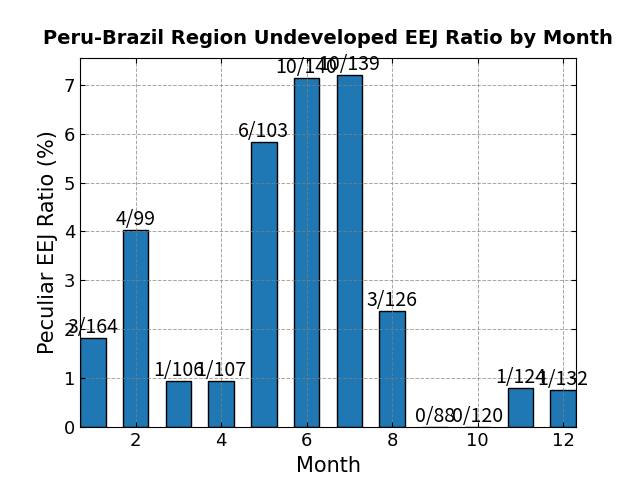
\includegraphics[width=\linewidth]{figures/2009-2020_peru_brazil_undeveloped_month.png}
    \caption{未発達型EEJの月ごとの発生割合（2009-2020年）}
    \label{fig:undeveloped_monthly}
  \end{minipage}
  \hfill
  \begin{minipage}{0.48\linewidth}
    \centering
    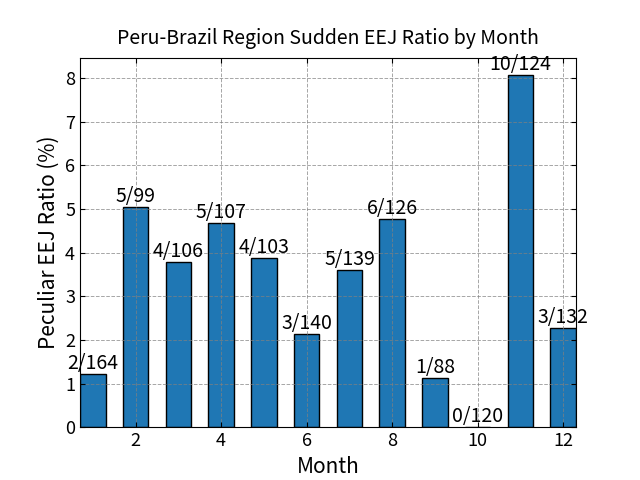
\includegraphics[width=\linewidth]{figures/2009-2020_peru_brazil_sudden_month.png}
    \caption{突発型EEJの月ごとの発生割合（2009-2020年）}
    \label{fig:sudden_monthly}
  \end{minipage}
\end{figure}


解析の結果、未発達型は南半球の冬至にあたるJ-solstice付近（5〜7月）において、発生率が高い傾向を示した。
具体的には、5月に103件中6件、6月に140件中10件、7月に139件中10件発生し、発生率のピークは7\%であった。
一方で、夏至にあたるD-solstice付近（11〜1月）においては、発生率が著しく減少していた。
11月は124件中1件、12月に132件中1件、1月に164件中2件発生し、発生率は約1\%であった。

突発型においては、9月と10月、1月において発生率が低いものの、11月に発生率が一番高く、前後の発生率を考慮すると、
平均して発生率は4\%程度であり、顕著な季節的な依存性はほとんどないように見ることができる。


\subsubsection{月潮汐効果との対応関係}
未発達型と突発型ごとの発生割合を図\ref{fig:undeveloped_lunar}、図\ref{fig:sudden_lunar}に示す。
\begin{figure}[htbp]
  \centering
  \begin{minipage}{0.48\linewidth}
    \centering
    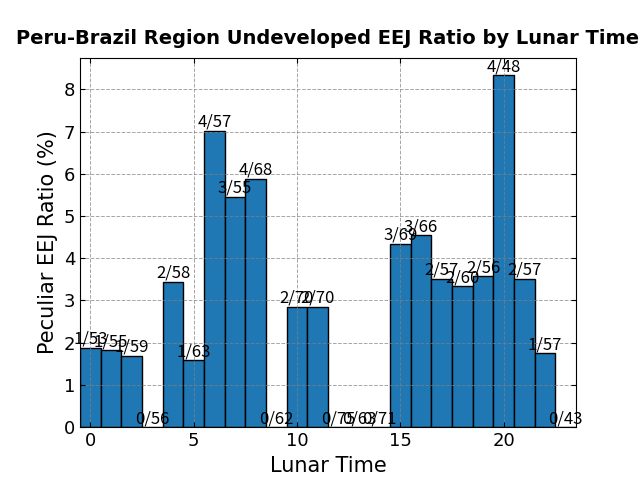
\includegraphics[width=\linewidth]{figures/2009-2020_peru_brazil_undeveloped_lunar.png}
    \caption{未発達型EEJの月齢ごとの発生割合（2009-2020年）}
    \label{fig:undeveloped_lunar}
  \end{minipage}
  \hfill
  \begin{minipage}{0.48\linewidth}
    \centering
    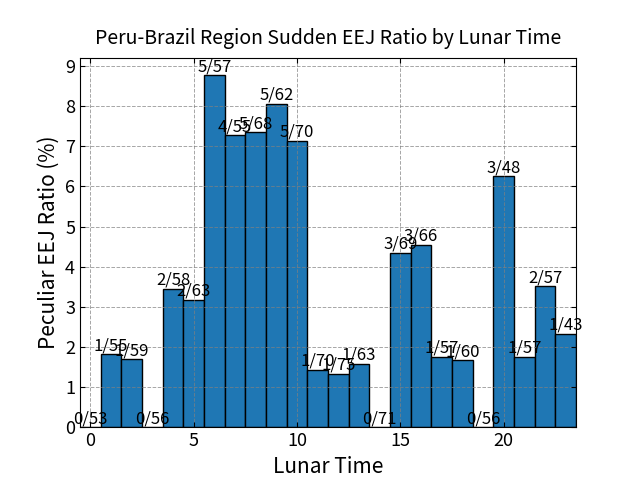
\includegraphics[width=\linewidth]{figures/2009-2020_peru_brazil_sudden_lunar.png}
    \caption{突発型EEJの月齢ごとの発生割合（2009-2020年）}
    \label{fig:sudden_lunar}
  \end{minipage}
\end{figure}

解析の結果、未発達型においては、Lunar age=6--9および15--21付近で高い傾向が見られた。
Lunar age=6--9では平均して発生率が6\%であり、Lunar age=15--21では平均して発生率が4\%であった。
一方Lunar age =0$\sim$5, 9$\sim$14, 22$\sim$24は発生率が低い傾向が見られ、発生率は1$\sim$3\%程度であった。


一方、突発型においては、Lunar age=6--10で高い傾向が見られ、7\%程度の発生率であった。
一方Lunar age=0$\sim$5, 11$\sim$14は発生率が低い傾向が見られ、1\%程度であった。


